%%%%%%%%%%%%%%%%%%%%%%%%%%%%%%%%%%%%%%%%%
% Programming/Coding Assignment
% LaTeX Template
%
% This template has been downloaded from:
% http://www.latextemplates.com
%
% Original author:
% Ted Pavlic (http://www.tedpavlic.com)
%
% Note:
% The \lipsum[#] commands throughout this template generate dummy text
% to fill the template out. These commands should all be removed when 
% writing assignment content.
%
% This template uses a Perl script as an example snippet of code, most other
% languages are also usable. Configure them in the "CODE INCLUSION 
% CONFIGURATION" section.
%
%%%%%%%%%%%%%%%%%%%%%%%%%%%%%%%%%%%%%%%%%

%----------------------------------------------------------------------------------------
%	PACKAGES AND OTHER DOCUMENT CONFIGURATIONS
%----------------------------------------------------------------------------------------

\documentclass{article}

\usepackage{fancyhdr} % Required for custom headers
\usepackage{lastpage} % Required to determine the last page for the footer
\usepackage{extramarks} % Required for headers and footers
\usepackage[usenames,dvipsnames]{color} % Required for custom colors
\usepackage{graphicx} % Required to insert images
\usepackage{listings} % Required for insertion of code
\usepackage{courier} % Required for the courier font
\usepackage{lipsum} % Used for inserting dummy 'Lorem ipsum' text into the template

\usepackage{float}
\usepackage{amsfonts}
\usepackage{amsmath}
\usepackage{bm}

% Margins
\topmargin=-0.45in
\evensidemargin=0in
\oddsidemargin=0in
\textwidth=6.5in
\textheight=9.0in
\headsep=0.25in

\linespread{1.1} % Line spacing

% Set up the header and footer
\pagestyle{fancy}
\lhead{K. Holmbeck and D. Tonne} % Top left header
\chead{\hmwkClass\ : \hmwkTitle} % Top center head
\rhead{\firstxmark} % Top right header
\lfoot{\lastxmark} % Bottom left footer
\cfoot{} % Bottom center footer
\rfoot{Page\ \thepage\ of\ \pageref{LastPage}} % Bottom right footer
\renewcommand\headrulewidth{0.4pt} % Size of the header rule
\renewcommand\footrulewidth{0.4pt} % Size of the footer rule

\setlength\parindent{0pt} % Removes all indentation from paragraphs

%----------------------------------------------------------------------------------------
%	CODE INCLUSION CONFIGURATION
%----------------------------------------------------------------------------------------

\usepackage{color} %red, green, blue, yellow, cyan, magenta, black, white
\definecolor{mygreen}{RGB}{28,172,0} % color values Red, Green, Blue
\definecolor{mylilas}{RGB}{170,55,241}

\lstset{language=Matlab,%
    basicstyle=\ttfamily\footnotesize,breaklines=true
    %basicstyle=\footnotesize\color{red},
    breaklines=true,%
    xleftmargin=0.5in,
    %xrightmargin=0.25in,
    morekeywords={matlab2tikz},
    keywordstyle=\color{blue},%
    morekeywords=[2]{1}, keywordstyle=[2]{\color{black}},
    identifierstyle=\color{black},%
    stringstyle=\color{mylilas},
    commentstyle=\color{mygreen},%
    showstringspaces=false,%without this there will be a symbol in the places where there is a space
    numbers=left,%
    numberstyle={\tiny \color{black}},% size of the numbers
    numbersep=9pt, % this defines how far the numbers are from the text
    emph=[1]{for,end,break},emphstyle=[1]\color{blue}, %some words to emphasise
    %emph=[2]{word1,word2}, emphstyle=[2]{style},    
}


%----------------------------------------------------------------------------------------
%	DOCUMENT STRUCTURE COMMANDS
%	Skip this unless you know what you're doing
%----------------------------------------------------------------------------------------

% Header and footer for when a page split occurs within a problem environment
\newcommand{\enterProblemHeader}[1]{
%\nobreak\extramarks{#1}{#1 continued on next page\ldots}\nobreak
%\nobreak\extramarks{#1 (continued)}{#1 continued on next page\ldots}\nobreak
}

% Header and footer for when a page split occurs between problem environments
\newcommand{\exitProblemHeader}[1]{
\nobreak\extramarks{#1 (continued)}{#1 continued on next page\ldots}\nobreak
\nobreak\extramarks{#1}{}\nobreak
}

\setcounter{secnumdepth}{0} % Removes default section numbers
\newcounter{homeworkProblemCounter} % Creates a counter to keep track of the number of problems

\newcommand{\homeworkProblemName}{}
\newenvironment{homeworkProblem}[1][Problem \arabic{homeworkProblemCounter}]{ % Makes a new environment called homeworkProblem which takes 1 argument (custom name) but the default is "Problem #"
\stepcounter{homeworkProblemCounter} % Increase counter for number of problems
\renewcommand{\homeworkProblemName}{#1} % Assign \homeworkProblemName the name of the problem
\subsection{\homeworkProblemName} % Make a section in the document with the custom problem count
\enterProblemHeader{\homeworkProblemName} % Header and footer within the environment
}{
\exitProblemHeader{\homeworkProblemName} % Header and footer after the environment
}

\newcommand{\problemAnswer}[1]{ % Defines the problem answer command with the content as the only argument
\noindent\framebox[\columnwidth][c]{\begin{minipage}{0.98\columnwidth}#1\end{minipage}} % Makes the box around the problem answer and puts the content inside
}

\newcommand{\homeworkSectionName}{}
\newenvironment{homeworkSection}[1]{ % New environment for sections within homework problems, takes 1 argument - the name of the section
\renewcommand{\homeworkSectionName}{#1} % Assign \homeworkSectionName to the name of the section from the environment argument
\subsection{\homeworkSectionName} % Make a subsection with the custom name of the subsection
\enterProblemHeader{\homeworkProblemName\ [\homeworkSectionName]} % Header and footer within the environment
}{
\enterProblemHeader{\homeworkProblemName} % Header and footer after the environment
}


%----------------------------------------------------------------------------------------
%   NAME AND CLASS SECTION
%----------------------------------------------------------------------------------------

\newcommand{\hmwkTitle}{Homework\ 5} % Assignment title
\newcommand{\hmwkDueDate}{Tuesday,\ May\ 8,\ 2018} % Due date
\newcommand{\hmwkClass}{Math\ 521} % Course/clas
\newcommand{\hmwkAuthorName}{Kristin Holmbeck} % Your name

%----------------------------------------------------------------------------------------
%   TITLE PAGE
%----------------------------------------------------------------------------------------

\title{
\textmd{\textbf{\hmwkClass \ \hmwkTitle}}\\
\normalsize\vspace{0.1in}\small{Due\ on\ \hmwkDueDate}\\
\vspace{0.1in}
\vspace{0.2in}
}

\author{\textbf{\hmwkAuthorName}}
\date{} % Insert date here if you want it to appear below your name

%----------------------------------------------------------------------------------------

\begin{document}

\maketitle

%----------------------------------------------------------------------------------------
%   TABLE OF CONTENTS
%----------------------------------------------------------------------------------------

%\setcounter{tocdepth}{1} % Uncomment this line if you don't want subsections listed in the ToC
\vspace{0.75in}
\tableofcontents
\listoffigures
\newpage

%----------------------------------------------------------------------------------------
%   PROBLEM 1
%----------------------------------------------------------------------------------------

% To have just one problem per page, simply put a \clearpage after each problem

\begin{section}{Theory}

\begin{homeworkSection}{1. Fourier series}
Suppose $f(w)$ has the Fourier series representation $f(w) = \sum_{k \in \mathbb{Z}} c_k e^{ikw}$ and suppose that $g(w) = e^{imw}f(w)$. For some $m \in \mathbb{Z}$, show that
$$
	g(w) = \sum_{k = -\infty}^{\infty} d_k e^{ikw}, \quad \text{where} \quad d_k = c_{k-m}
$$
\\
\problemAnswer{
}
\end{homeworkSection}

\begin{homeworkSection}{2. Fourier series}
Find the Fourier series for the $2\pi$-periodic square wave function 
$$
	f(\omega) = \left \lbrace \begin{matrix} -k && \text{if} && -\pi < \omega < 0\\
		k && \text{if} && 0 < \omega < \pi \\
	 \end{matrix} \right.
	\quad \text{and} \quad f(\omega + 2\pi) = f(\omega)
$$
\\
\problemAnswer{
}
\end{homeworkSection}

\begin{homeworkSection}{3. Wavelet decomposition}
Compute by hand the Haar wavelet decomposition (Pyramidal decomposition) of the vector $x^T = [1,7,−3,2]$ by viewing it as
$$
	f(x) = \left \lbrace 
	\begin{matrix} 
		1 && \text{if} && x \in [0,\frac{1}{4}) \\
		7 && \text{if} && x \in [\frac{1}{4}, \frac{1}{2}) \\
		-3 && \text{if} && x \in [\frac{1}{2},\frac{3}{4}) \\
		2 && \text{if} && x \in [\frac{3}{4},1) \\
	 \end{matrix} \right.
	\quad \text{and} \quad f(\omega + 2\pi) = f(\omega)
$$
Graphically show the projections onto the scaling and wavelet subspaces
\\
\\
\problemAnswer{ 
}
\end{homeworkSection}

\begin{homeworkSection}{3. }
Let $\bm{x} \in \mathbb{R}^M$, and let $\bm{y}$ be the 1D DWT of $\bm{x}$. If we write the Haar wavelet transform and its inverse as matrix operations, i.e.
$$ \bm{y} = W \bm{x} $$ and $$ \bm{x} = \tilde{W} \bm{y},$$
what are $W$ and $\tilde{W}$? This should be done in terms of the Haar Pyramidal Decomposition algorithm, i.e., the expressions of $W$ and $\tilde{W}$ depend on the level of the decomposition/reconstruction. If
\\ $\bm{x} = [576,704,1152,1280,1344,1472,1536,1536]$, what is its Haar wavelet transform after 3 ($2^3 = 8$) levels of decompositions?
\\
\\
\problemAnswer{ 
}
\end{homeworkSection}

\end{section}


\begin{section}{Computing}
\begin{homeworkSection}{1. }
Implement a $3 \times 3$ \textit{median filter} and apply the filtering  process on a corrupted image of “app-ndt-Chip5.JPG”
located via the course website. Specifically, corrupt “app-ndt-Chip-5.JPG” with \textit{salt-and-pepper} noise, where the corrupted pixels are either set to the maximum value (which looks like snow in the image) or have single bits flipped over. In some cases, single pixels can be set alternatively to zero or to the maximum value (i.e., 255 on a 8-bit machine). Then apply the median filter to de-noise the corrupted image. Compare your result with the original.
\end{homeworkSection}

\begin{homeworkSection}{2. }
Given an image “CTimage.JPG“ on the course website, perform the following operations:
\renewcommand{\theenumi}{\alph{enumi}}
\begin{enumerate}
	\item Construct a $3 \times 3$ average filter to smooth the image.
	\item Then use a 2D Laplacian filter mask to extract the edges of the smoothed image.
	\item Finally, enhance the smoothed image with the result from part (b). How does this image compare to the original?
\end{enumerate}
\end{homeworkSection}

\begin{homeworkSection}{3. }
Write a \textsc{MATLAB} code to implement the 1D Discrete Haar Wavelet Transform (1D HWT) including the algorithms for
\begin{itemize}
	\item Haar pyramidal decomposition, and
	\item Haar pyramidal reconstruction
\end{itemize}
Compute the six-level decomposition of the data
$$ f_n = \sin \left ( \frac{n^2}{10,000} \right ) + \nu_n, $$
where $n = 1,\ldots,1024$, and $\nu_n$ is  selected from a normal distribution with mean zero and variance 0.2 (see figure below). Initialize the transform by assuming that $\bm{f} \in V_0$. Include the following plots in your report:
\renewcommand{\theenumi}{\alph{enumi}}
\begin{enumerate}
	\item $P_i \bm{f} = \bm{f}^i_a \in V_i$ for all $i = 1, \ldots, 6$.
	\item $Q_i \bm{f} = \bm{f}^i_d \in W_i$ for all $i = 1, \ldots, 6$.
\end{enumerate}
Be sure that each plot has domain [1,1024].
\\
\begin{center}
\begin{minipage}{0.5\textwidth}
    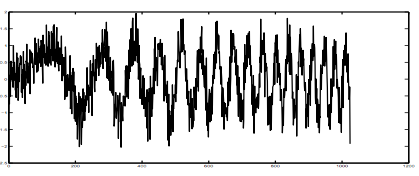
\includegraphics[trim={0cm 0cm 0cm 0cm},clip,width=1.0\columnwidth]{tmp}
\end{minipage}
\end{center}
\end{homeworkSection}

\begin{homeworkSection}{4. }
Test your codes with your favorite image for this problem. Make sure your codes are as general as possible and be sure to plot the results.
\renewcommand{\theenumi}{\alph{enumi}}
\begin{enumerate}
	\item Write a function in \textsc{MATLAB} to compute the approximation and each of the three detail components of an image. (i.e., you will produce 4 \textit{extremely} short codes here) Notice that the resolution of LL, HL, LH, and HH will be $M/2 \times N/2$, where $(M,N)$ is the resolution of the original image.
	\item Write a subroutine to reconstruct an image from \textbf{only} the approximation component as a function of level. Notice that the resolution of the reconstructed image will be of size $M\times N$.
	\item Compress the image up to level 3 using \textbf{only the approximation component}. Compute the compression ratio as a function of each compression level. Plot the compressed image for each level along with their compression ratio. Note that the compression ratio in this case can be defined as
	$$
		CR = \frac{ \text{\# of nonzero entries in the original} }{ \text{\# of nonzero entries in the compressed} }
	$$
\end{enumerate}
\end{homeworkSection}

\end{section}

%----------------------------------------------------------------------------------------
\newpage

\appendix

\section{Code}\label{code}

%\subsection{Gram-Schmidt} \label{code:gram_schmidt}
%\lstinputlisting{../Kristin_Holmbeck_HW2_GramSchmidt.m}


\begin{thebibliography}{10}
    \bibitem{chang}
    Chang, Jen-Mei. \textit{Matrix Methods for Geometric Data Analysis and Recognition}. 2014.

\end{thebibliography}

\end{document}
